\chapter{Musical Notes}

\section{Aim}
To investigate the relationship between the length and tension of a string and the frequency of its sound

\section{Background Information}
Have you ever wondered why a guitar can make so many different sounds from only five strings? The brain distinguishes different sound waves by their frequencies. A high frequency (high pitch) sound wave sounds different to us than a low frequency (low pitch) sound wave. This means that the guitar is able to produce a range of frequencies from these strings. Thus, there must be some relationship between the string and the frequency of the sound it produces. What is this relationship?

\section{Materials}
Sonometer, masses, mass hanger, and a peg

\section{Procedure}
\begin{enumerate}
\item Pass the wire over the pulley as seen in the figure.
\item Hang masses on a mass hanger which is attached to the loose end of the wire until the wire becomes taut.
\item Pluck the string in the middle and listen to the sound. 
\item Repeat procedure (3) after moving the bridges closer together. Do this for 4 different intervals of distance between the bridges. 
\item Return the bridges to their original positions. 
\item Increase the amount of mass on the mass hanger and pluck the string again. Listen to the sound.
\item Repeat procedure (6) four more times using increased mass on the hanger each time.
\end{enumerate}

\begin{figure}[h!]
\centering
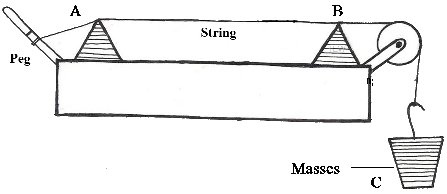
\includegraphics[width=14cm]{./img/musical-notes-1.png}
\caption{Musical Notes practical setup}
\label{fig:musical-notes-1}
\end{figure}

\section{Analysis and Interpretation}
\begin{enumerate}
\item What did you observe about the sound from the string when the distance between the bridges was decreased?
\item What did you observe about the sound from the string when the weight on string increased?
\end{enumerate}

\section{Conclusion}
What is the relationship between the length and tension of a string and the frequency of the sound wave it produces?

\section{Questions for Discussion}
\begin{enumerate}
\item If you kept the length and tension of the string constant, but used a thicker string, (i.e. more massive), do you expect to hear a change in the frequency of the sound?
\item What would happen if there were no tension on the string?
\end{enumerate}

\section{Reflection and Self Assessment}
\begin{enumerate}
\item Is there anything you do not understand in this experiment? If so, what and in what ways can you increase your understanding?
\item How can you use the results of this experiment in your daily life?
\end{enumerate}